\section{Software Design}

\subsection{High-Level Architecture (textual)}
Five-layer architecture (as in SRS) — component view and interaction flow.

\textbf{Interaction flow (short):}
\begin{quote}
Client $\rightarrow$ API Gateway $\rightarrow$ Chat Engine $\rightarrow$ (Intent Classifier $\rightarrow$ RAG Retrieval + LLM) $\rightarrow$ Response $\rightarrow$ Presentation.
\end{quote}

Escalation path sends conversation + context to Human Agent Dashboard; Human updates KB via Admin Service.

\subsection{Component/Service Summary}
Below are the top-level services (each top-level class may map to a microservice).

\begin{itemize}
  \item \textbf{APIGateway} — Authentication, rate-limiting, routing, request validation.
  \item \textbf{ChatEngine} — Orchestrates conversational processing, session management, calls ML services.
  \item \textbf{AdminService} — KB CRUD, guardrails, role management.
  \item \textbf{HumanDashboard} (HumanAgent) — Agent UI/API for escalations and KB updates.
  \item \textbf{AnalyticsService} — Logs metrics, calculates KPIs, anomaly alerts.
  \item \textbf{IntentClassifier} — Predicts intent/domain with confidence scores.
  \item \textbf{MultimodalProcessor} — Image OCR, document classification, entity extraction.
  \item \textbf{RAGEngine} — Vector search + LLM prompt generation and answer synthesis.
  \item \textbf{DataStore} — Relational DB (Postgres), vector store (FAISS/Milvus/Elastic vectors), cache (Redis).
\end{itemize}

\subsection{UML}
Below is a UML diagram describing the UML class/service relationships.
\begin{figure}[h!]
    \centering
    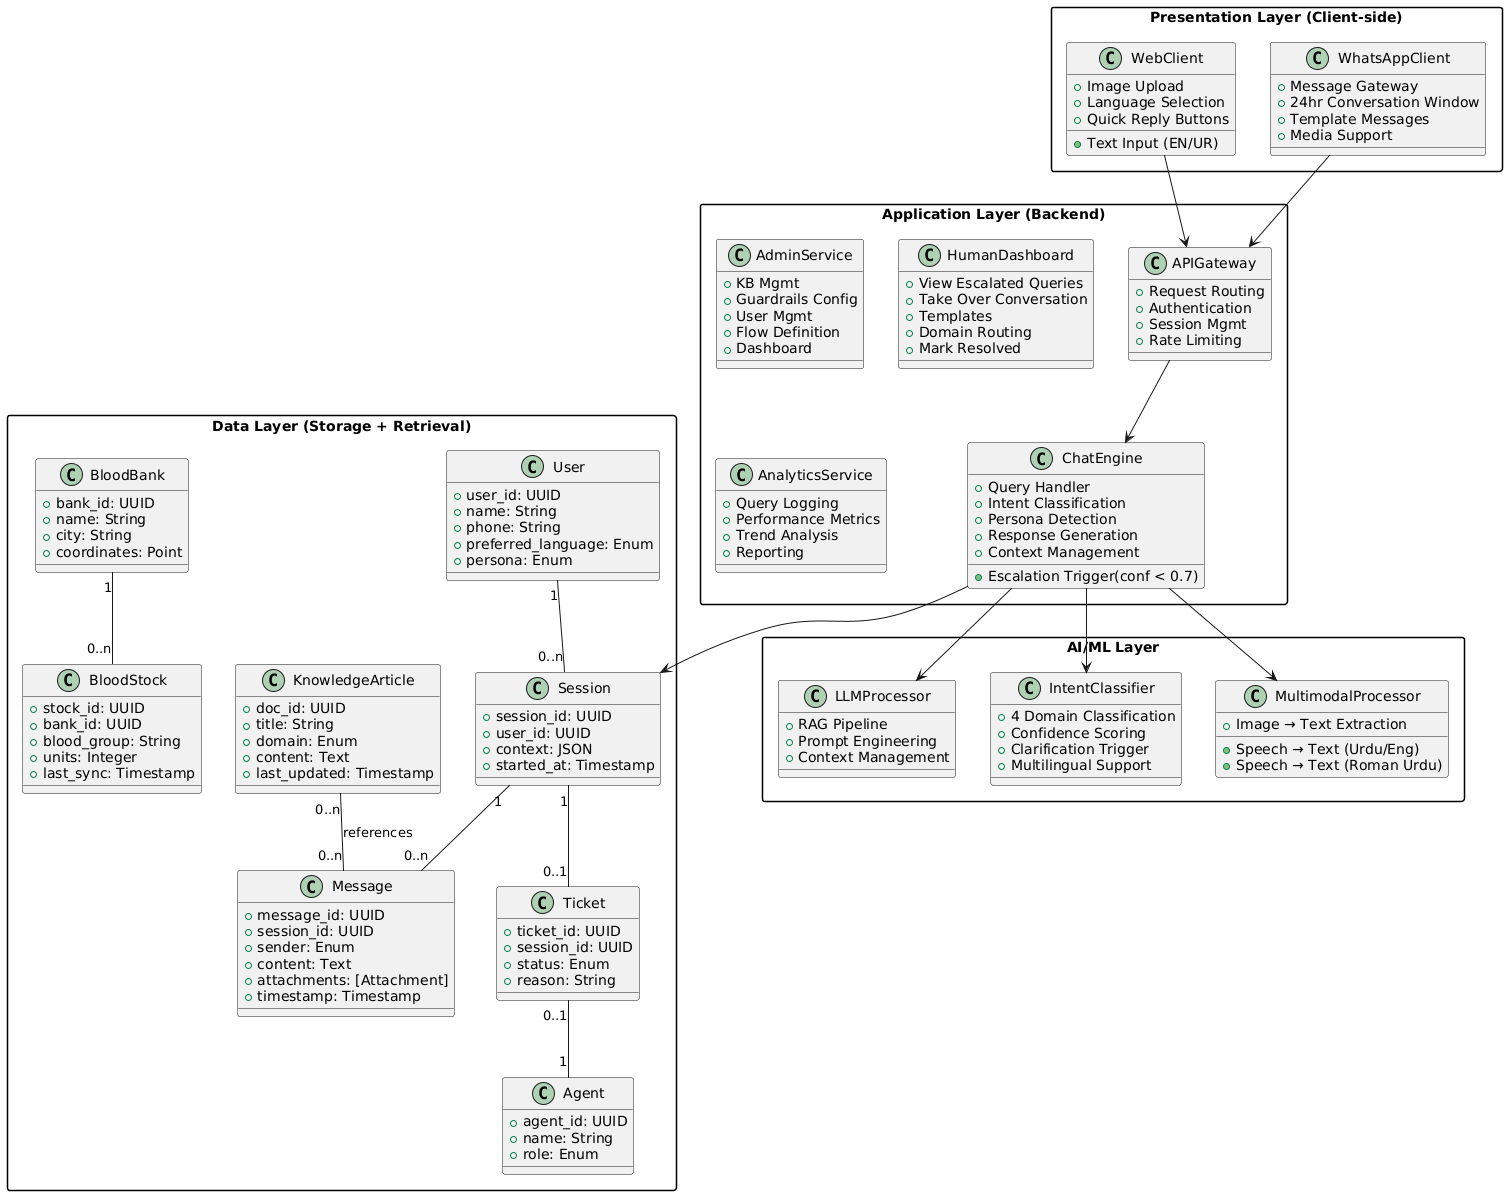
\includegraphics[width=0.95\linewidth]{chapters/UML.png}
    \caption{UML Diagram}
    \label{fig:placeholder}
\end{figure}
\subsection{Classes - Descriptions}
Below are concise descriptions, attributes and methods for the main classes/services.

\subsubsection{APIGateway}
\textbf{Purpose:} Authentication, rate-limiting, routing to backend services, request validation.  
\textbf{Attributes:} tokenStore (JWT secret), rateLimitConfig.  
\textbf{Methods:} \texttt{authenticate(req)}, \texttt{authorize(req)}, \texttt{route(req)}, \texttt{rateLimit(req)}.  
\textbf{Relationships:} front door for WebClient \& WhatsAppClient $\rightarrow$ ChatEngine, AdminService.

\subsubsection{ChatEngine}
\textbf{Purpose:} Orchestrates conversational processing: receives messages, manages sessions, calls intent classifier, multimodal processor, RAG engine, returns responses and handles escalation.  
\textbf{Attributes:} sessionStore (Redis), kbClient, classifierClient, ragClient, escalationPolicy.  
\textbf{Methods:}
\begin{itemize}
  \item \texttt{processIncoming(message: Message)}
  \item \texttt{classifyIntent(text) $\rightarrow$ IntentResult}
  \item \texttt{handleMultimodal(attachments) $\rightarrow$ structured artifacts}
  \item \texttt{generateResponse(context) $\rightarrow$ final message}
  \item \texttt{escalate(session, reason) $\rightarrow$ creates Ticket}
\end{itemize}
\textbf{Relationships:} calls IntentClassifier, MultimodalProcessor, RAGEngine, DataStore.

\subsubsection{AdminService}
\textbf{Purpose:} CRUD for knowledge base, guardrails, role management.  
\textbf{Attributes:} KBRepository, userManager.  
\textbf{Methods:} \texttt{createArticle()}, \texttt{updateArticle()}, \texttt{publishKBVersion()}, \texttt{setGuardrails()}.

\subsubsection{HumanDashboard}
\textbf{Purpose:} Staff-facing UI/API for taking over escalated tickets, replying to users, updating KB.  
\textbf{Attributes:} ticketQueue, websocketConnections.  
\textbf{Methods:} \texttt{claimTicket(ticketId)}, \texttt{postReply(ticketId, message)}, \texttt{updateKBFromInteraction(...)}.

\subsubsection{AnalyticsService}
\textbf{Purpose:} Log metrics, build KPIs.  
\textbf{Attributes:} metricsStore, logDB.  
\textbf{Methods:} \texttt{logQuery(...)} , \texttt{getKPI(start,end)}, \texttt{alertAnomalies()}.

\subsubsection{AI/ML Services}
\textbf{IntentClassifier:} model (transformer or embed+classifier), \texttt{predict(text)} $\rightarrow$ \{intent, domain, confidence, top\_k\}.  
\textbf{MultimodalProcessor:} visionModel, ocrEngine, imagePreproc, \texttt{processImage(img)}.  
\textbf{RAGEngine:} vectorStore, index, llmClient, promptTemplates, \texttt{retrieve(query,k)}, \texttt{buildPrompt(context, docs)}, \texttt{generateAnswer(prompt)}.

\subsubsection{Data-layer domain models}
\textbf{User, Session, Message, Ticket, KnowledgeArticle, Agent, BloodBank, BloodStock, AuditLog} — attributes and typical service-level methods (getProfile, loadContext, serialize, assign, resolve, searchIndex).

\section{Data Design}

\subsection{Entities, PK/FK and Cardinalities (summary)}
\begin{itemize}
  \item \textbf{User (1) -- (0..n) Session} : A user can have many sessions.
  \item \textbf{Session (1) -- (0..n) Message} : A session has many messages.
  \item \textbf{Session (1) -- (0..1) Ticket} : A session may create a ticket.
  \item \textbf{Ticket (0..n) -- (0..1) Agent} : Tickets can be assigned to an agent.
  \item \textbf{KnowledgeArticle (0..n) -- (0..n) Message} : Many-to-many via junction table message\_article\_refs.
  \item \textbf{BloodBank (1) -- (0..n) BloodStock} : Each bank has multiple stock entries.
\end{itemize}

\subsection{Relational Schema (core tables) — SQL DDL}
Below are simplified Postgres table definitions for core tables. In production add indexes, constraints, partitioning, and tuning.

\begin{lstlisting}[language=SQL]
-- Users
CREATE TABLE users (
  user_id UUID PRIMARY KEY,
  name TEXT,
  phone TEXT,
  email TEXT,
  preferred_language TEXT,
  created_at TIMESTAMP WITH TIME ZONE DEFAULT now()
);

-- Sessions
CREATE TABLE sessions (
  session_id UUID PRIMARY KEY,
  user_id UUID REFERENCES users(user_id),
  started_at TIMESTAMP WITH TIME ZONE DEFAULT now(),
  last_active_at TIMESTAMP WITH TIME ZONE DEFAULT now(),
  context JSONB
);

-- Messages
CREATE TABLE messages (
  message_id UUID PRIMARY KEY,
  session_id UUID REFERENCES sessions(session_id) ON DELETE CASCADE,
  sender TEXT,
  content TEXT,
  attachments JSONB,
  timestamp TIMESTAMP WITH TIME ZONE DEFAULT now(),
  intent_label TEXT,
  confidence NUMERIC
);

-- Tickets
CREATE TABLE tickets (
  ticket_id UUID PRIMARY KEY,
  session_id UUID REFERENCES sessions(session_id),
  status TEXT,
  assigned_to UUID, -- references agents.agent_id (create agents table below)
  priority TEXT,
  reason TEXT,
  created_at TIMESTAMP WITH TIME ZONE DEFAULT now(),
  resolved_at TIMESTAMP WITH TIME ZONE
);

-- Knowledge articles
CREATE TABLE knowledge_articles (
  doc_id UUID PRIMARY KEY,
  title TEXT,
  content TEXT,
  domain TEXT,
  tags TEXT[],
  source_url TEXT,
  last_updated TIMESTAMP WITH TIME ZONE,
  version INTEGER
);

-- Message <-> Article references (junction)
CREATE TABLE message_article_refs (
  id UUID PRIMARY KEY,
  message_id UUID REFERENCES messages(message_id),
  doc_id UUID REFERENCES knowledge_articles(doc_id)
);

-- Agents
CREATE TABLE agents (
  agent_id UUID PRIMARY KEY,
  name TEXT,
  roles TEXT[],
  email TEXT,
  active BOOLEAN DEFAULT true
);

-- Blood bank and stock
CREATE TABLE blood_banks (
  bank_id UUID PRIMARY KEY,
  name TEXT,
  address TEXT,
  city TEXT,
  coordinates POINT,
  contact TEXT
);

CREATE TABLE blood_stock (
  stock_id UUID PRIMARY KEY,
  bank_id UUID REFERENCES blood_banks(bank_id) ON DELETE CASCADE,
  blood_group TEXT,
  units_available INTEGER,
  last_updated TIMESTAMP WITH TIME ZONE
);
-- Unique constraint to prevent duplicate (bank_id, blood_group)
ALTER TABLE blood_stock
  ADD CONSTRAINT uniq_bank_group UNIQUE (bank_id, blood_group);

-- Audit logs
CREATE TABLE audit_logs (
  log_id UUID PRIMARY KEY,
  actor_id UUID,
  action TEXT,
  details JSONB,
  timestamp TIMESTAMP WITH TIME ZONE DEFAULT now()
);
\end{lstlisting}

\subsection{Indexes and Search}
\begin{itemize}
  \item Full-text search: add \texttt{tsvector} columns and GIN indexes on \texttt{knowledge\_articles(content, title)}.
  \item Vector embeddings: store in a vector store (FAISS/Milvus/Elastic vector index) keyed by \texttt{doc\_id}. Keep metadata in a \texttt{kb\_index} table linking \texttt{doc\_id} $\rightarrow$ vector\_id.
  \item Cache hot items in Redis. Use LRU eviction for cache.
\end{itemize}

\subsection{Normalization \& Cardinalities Rationale}
Schema is in 3NF:
\begin{itemize}
  \item KB articles separated from message-level references to avoid duplication.
  \item Sessions store transient conversation context; messages are transactional and cascade on session deletion.
  \item Blood\_stock uses unique constraint on (bank\_id, blood\_group) to avoid duplication and simplify updates.
  \item message\_article\_refs preserves KB provenance for each response.
\end{itemize}

\section{Technical Details — Algorithms \& Implementation Notes}

For each pipeline I list purpose, inputs/outputs, steps (pseudocode), placement, complexity, failure modes and mitigations.

\subsection{Incoming Message Pipeline (Orchestration)}
\textbf{Purpose:} End-to-end handling of a user message: preproc $\rightarrow$ intent $\rightarrow$ retrieval/generation $\rightarrow$ response or escalate.  
\textbf{Placement:} ChatEngine service.

\textbf{Input:} Message (text + optional attachments + user\_id + session\_id).  
\textbf{Output:} Response (text, attachments, metadata), or created Ticket.

\textbf{Pseudocode:}
\begin{lstlisting}
function processIncoming(msg):
  session = SessionStore.get(msg.session_id)
  preproc_text = normalize_text(msg.content, user_lang=session.pref_lang)
  if msg.attachments present:
    image_info = MultimodalProcessor.process(msg.attachments)
    enrich context with image_info

  intent_result = IntentClassifier.predict(preproc_text)
  if intent_result.confidence < CONFIDENCE_THRESHOLD (0.7):
    create_ticket(session, reason='low_confidence', msg)
    return respond_with_escalation_notice()
  
  docs = RAGEngine.retrieve(preproc_text, k=5)
  prompt = RAGEngine.buildPrompt(session.context, preproc_text, docs)
  answer, sources = RAGEngine.generateAnswer(prompt)
  
  persona = PersonaService.get(session.user_id)
  answer = PersonaService.format(answer, persona)
  
  Analytics.log(query, intent_result, latency)
  MessageStore.saveBotResponse(session, answer, sources)
  return answer
\end{lstlisting}

\textbf{Complexity:} Vector retrieval typically sub-linear; LLM generation dominates latency and cost.  
\textbf{Failure modes:} LLM hallucination, outdated KB — mitigate by returning explicit sources, confidence, and allowing human escalation.

\subsection{Intent Classification}
\textbf{Purpose:} Route queries by domain and decide escalation.

\textbf{Options:}
\begin{description}
  \item[Option A (recommended):] Transformer fine-tuned classifier (small BERT / DistilBERT) for multilingual support.
  \item[Option B:] Embedding + k-NN for low-resource scenarios.
\end{description}

\textbf{Pseudocode:}
\begin{lstlisting}
predict(text):
  tokens = tokenizer(text)
  probs = model.forward(tokens)  -- softmax per class
  label = argmax(probs)
  confidence = probs[label]
  return {label, confidence}
\end{lstlisting}

\textbf{Notes:} Confidence threshold = 0.7. Return top\_k candidate intents for clarification loops. Use data augmentation for Roman Urdu.

\subsection{RAG Retrieval \& Generation Pipeline}
\textbf{Purpose:} Factually-grounded LLM responses using KB documents.

\textbf{Steps:}
\begin{enumerate}
  \item Preprocess query (language, entity extraction).
  \item Embed query; vector search top-k (k=5--10).
  \item Rerank by metadata (city, blood group, last\_updated).
  \item Build structured prompt with system instruction + context + doc excerpts + provenance.
  \item Call LLM to generate answer.
  \item Post-process: sanitize, attach citations, compute heuristic confidence.
\end{enumerate}

\textbf{Pseudocode:}
\begin{lstlisting}
docs = vector_search(query, k)
docs = rerank_by_metadata(docs, query_entities)
prompt = build_prompt(context, query, docs)
answer = llm.generate(prompt)
sources = extract_sources(answer, docs)
\end{lstlisting}

\textbf{Notes:} Use chunking for long docs, prioritize recently-updated docs for time-sensitive queries (e.g., blood availability). Add guardrails to prevent PII exposure.

\subsection{Multimodal Processing (Image Handling)}
\textbf{Purpose:} Extract text and structured info from images (receipts, prescriptions, confirmations).

\textbf{Steps:}
\begin{itemize}
  \item Preprocess image (resize, denoise).
  \item Doc-type classification: CNN predicts receipt/prescription/ID/photo.
  \item Run OCR (Tesseract or cloud).
  \item Entity extraction: NER or regex on OCR text (txn\_id, date, hospital).
  \item Return structured JSON to ChatEngine.
\end{itemize}

\textbf{Limitations:} Handwritten recognition out-of-scope for MVP; low-quality images return low-confidence and prompt user to reupload.

\subsection{Persona Classification \& Response Personalization}
\textbf{Purpose:} Tailor tone, verbosity, and suggestions based on the persona (donor type, patient type).

\textbf{Technique:} Rule-based + light ML classifier using session history, language, frequency. Persona stored in Redis or persona\_profile table.

\subsection{Escalation Logic (Human Handoff)}
\textbf{Purpose:} Move low-confidence or sensitive queries to human agents preserving context.

\textbf{Rules:}
\begin{itemize}
  \item intent.confidence < 0.7 $\rightarrow$ escalate.
  \item Sensitive patterns (refund, complaint, PII requests) $\rightarrow$ escalate.
  \item user explicitly requests human $\rightarrow$ escalate.
\end{itemize}

\textbf{Steps:}
\begin{enumerate}
  \item Create ticket with snapshot context.
  \item Notify agent queue (domain-based).
  \item Lock session for human takeover.
  \item Agent replies via Dashboard; ChatEngine relays reply.
  \item Agent may update KB \& resolve ticket.
\end{enumerate}

\subsection{Session Management \& Context Windowing}
\textbf{Purpose:} Maintain multi-turn context while staying below LLM prompt limits.

\textbf{Technique:} Keep full short context in Redis; for long histories summarize early messages into compact structured fields (last\_intent, open\_issues, recent\_entities) and include recent N messages directly.

\subsection{Caching \& Performance}
\textbf{Layers:}
\begin{itemize}
  \item Redis: sessions, persona, short-term query cache.
  \item Persistent cache / warm vector cache: frequently-seen RAG results (TTL e.g., 1h).
\end{itemize}

\textbf{Scaling:} Containerize services horizontally. Vector store and Elasticsearch scaled/sharded as needed.

\subsection{Monitoring, Logging, Analytics}
\textbf{Metrics:} QPS, avg latency, LLM call latency, intent accuracy, escalation rate, KB hit rate, user satisfaction.  
\textbf{Tools:} Prometheus (metrics), Grafana (dashboards), ELK (logs).  
\textbf{Alerts:} High escalation rate, low accuracy, traffic spikes.

\subsection{Data Integrity, Backup \& Compliance}
\begin{itemize}
  \item Weekly snapshots for KB \& relational DB, daily incremental backups for messages/tickets.
  \item Off-site encrypted backups.
  \item Pseudonymize or avoid persisting PII unless explicit consent.
  \item RBAC for Admin/Agent, audit logs required for agent actions.
  \item Follow local data protection rules.
\end{itemize}

\subsection{Security Design}
\begin{itemize}
  \item TLS everywhere.
  \item JWT for session tokens; secrets in a vault.
  \item Input sanitization for prompts; escape user-supplied data.
  \item Rate-limiting; WhatsApp 24-hour window compliance (templates/outbound).
  \item LLM guardrails to block medical diagnoses and PII disclosure.
\end{itemize}

\section{Example Sequence: ``Find nearest blood bank with O+ in Karachi''}
Example interaction flow:
\begin{enumerate}
  \item User: ``I need O+ blood in Karachi now'' (WhatsApp).
  \item APIGateway authenticates request.
  \item ChatEngine retrieves/creates session.
  \item IntentClassifier $\rightarrow$ BloodService (confidence 0.95).
  \item Entities: blood\_group=O+, city=Karachi.
  \item RAGEngine queries BloodStock microservice (filter: city, blood\_group) $\rightarrow$ nearby\_banks[] with availability.
  \item RAGEngine builds reply with nearest banks, contacts, estimated distances, and a quick-action button.
  \item Message sent to user; analytics logged. If stock below threshold, system triggers donor network alert.
\end{enumerate}

\section{Additional Implementation Notes \& Trade-offs}
\begin{itemize}
  \item \textbf{LLM choice:} Local LLaMA2 (privacy, cost) vs hosted OpenAI (language capability). For Urdu/Roman Urdu, RAG may compensate for smaller LLMs.
  \item \textbf{Vector store:} Elastic vector index or FAISS/Milvus; real-time stock requires streaming updates to metadata or direct DB queries.
  \item \textbf{Multilingual support:} Roman Urdu normalization tables, data augmentation.
  \item \textbf{Latency vs accuracy:} Use caching, smaller prompts to lower latency; accept higher latency for complex answers.
  \item \textbf{Human-in-loop:} Agent UX to push KB updates from interactions to keep RAG fresh.
\end{itemize}

\section{Deliverables Usable in Implementation}
\begin{itemize}
  \item PlantUML file (above) — drop-in to generate UML diagram.
  \item SQL DDL (above) — base schema for Postgres.
  \item Pseudocode for pipelines — can be translated into FastAPI + background workers.
  \item Metrics list — ready for Prometheus instrumentation.
\end{itemize}

\section{Risks and Mitigations}
\begin{itemize}
  \item \textbf{Outdated KB:} show last\_updated timestamps; explicit sources; escalate to humans.
  \item \textbf{Roman Urdu variability:} curated normalization and data augmentation.
  \item \textbf{WhatsApp 24-hour window:} use pre-approved templates; agents respect window.
  \item \textbf{Privacy risks:} minimal PII storage, anonymize logs, strong access controls and encryption.
\end{itemize}

\section{Appendices}

\subsection{Appendix A: Process Pseudocode (processIncoming \& escalate)}
\begin{lstlisting}
-- processIncoming (high-level)
function processIncoming(msg):
  session = SessionStore.get(msg.session_id)
  preproc_text = normalize_text(msg.content, user_lang=session.pref_lang)
  if msg.attachments:
    image_info = MultimodalProcessor.process(msg.attachments)
    session.context.enrich(image_info)

  intent_result = IntentClassifier.predict(preproc_text)
  if intent_result.confidence < THRESHOLD:
    ticket = EscalationRouter.createTicket(session, reason='low_confidence', msg=msg)
    return { type: 'escalation', ticket_id: ticket.id }

  docs = RAGEngine.retrieve(preproc_text, k=5)
  prompt = RAGEngine.buildPrompt(session.context, preproc_text, docs)
  answer, sources = RAGEngine.generateAnswer(prompt)

  persona = PersonaService.get(session.user_id)
  final_answer = PersonaService.format(answer, persona)

  Analytics.log({ query: preproc_text, intent: intent_result, latency: measured_latency })
  MessageStore.saveBotResponse(session, final_answer, sources)
  return final_answer

-- escalate
function escalate(session, reason, snapshot):
  ticket = TicketDB.create({
    session_id: session.session_id,
    reason: reason,
    snapshot: snapshot,
    status: 'Open',
    created_at: now()
  })
  EscalationRouter.notifyAgentQueue(ticket)
  AuditLog.create(actor='system', action='escalate', details={ticket_id: ticket.id, reason: reason})
  return ticket
\end{lstlisting}

\subsection{Appendix B: Example SQL Index Recommendations}
\begin{lstlisting}
-- Example indexes
CREATE INDEX idx_sessions_user ON sessions(user_id);
CREATE INDEX idx_messages_session_time ON messages(session_id, timestamp);
CREATE INDEX idx_articles_tsv ON knowledge_articles USING GIN (to_tsvector('english', title || ' ' || content));
CREATE INDEX idx_blood_stock_city_group ON blood_stock USING btree (blood_group);
\end{lstlisting}

\subsection{Appendix C: Notes on Performance}
\begin{itemize}
  \item LLM call latency will dominate both cost and time. Consider caching frequent queries and smaller dedicated models for intent-only tasks.
  \item Vector search scales with appropriate indexing; FAISS/Milvus provide fast ANN retrieval.
  \item Use async workers to precompute embeddings on KB updates.
\end{itemize}

\section{Next steps (suggested)}
If you'd like, I can:
\begin{enumerate}
  \item export the PlantUML above into a downloadable `.puml` file,
  \item produce a complete exportable SQL file with full indexes, constraints and sample seed data,
  \item generate example FastAPI endpoints and detailed pseudocode for \texttt{processIncoming} and \texttt{escalate} functions (including code snippets),
  \item or convert this LaTeX to a ready-to-download PDF.
\end{enumerate}

\bigskip
\noindent Thank you — tell me which of the above you'd like next or if you want specific sections expanded (for example, a detailed sequence diagram, ER diagram PNG, or production deployment diagram).
\end{document}
